%! Author = Raffaele
%! Date = 17/01/2024

\newpage
\thispagestyle{headings}
\section{Schema dell'architettura}\label{sec:Schema}
L'architettura del progetto è basata su una rete P2P puramente decentralizzata, in quanto
tutti i nodi sono uguali, sebbene quantitativamente piccola: \\
I due giocatori costituiscono i \textbf{Peer}, poiché svolgono la funzione sia di
client che di server: entrambi devono notificare immediatamente la controparte riguardo
i movimenti della propria racchetta, inoltre l'ultimo giocatore che ha toccato la pallina deve fare
da \textit{seeder}, deve cioè calcolare il movimento della pallina e comunicarlo alla controparte.
Il seeder si occupa anche di aggiornare il punteggio e di comunicarlo all'altro giocatore.

\begin{figure}
    \centering
    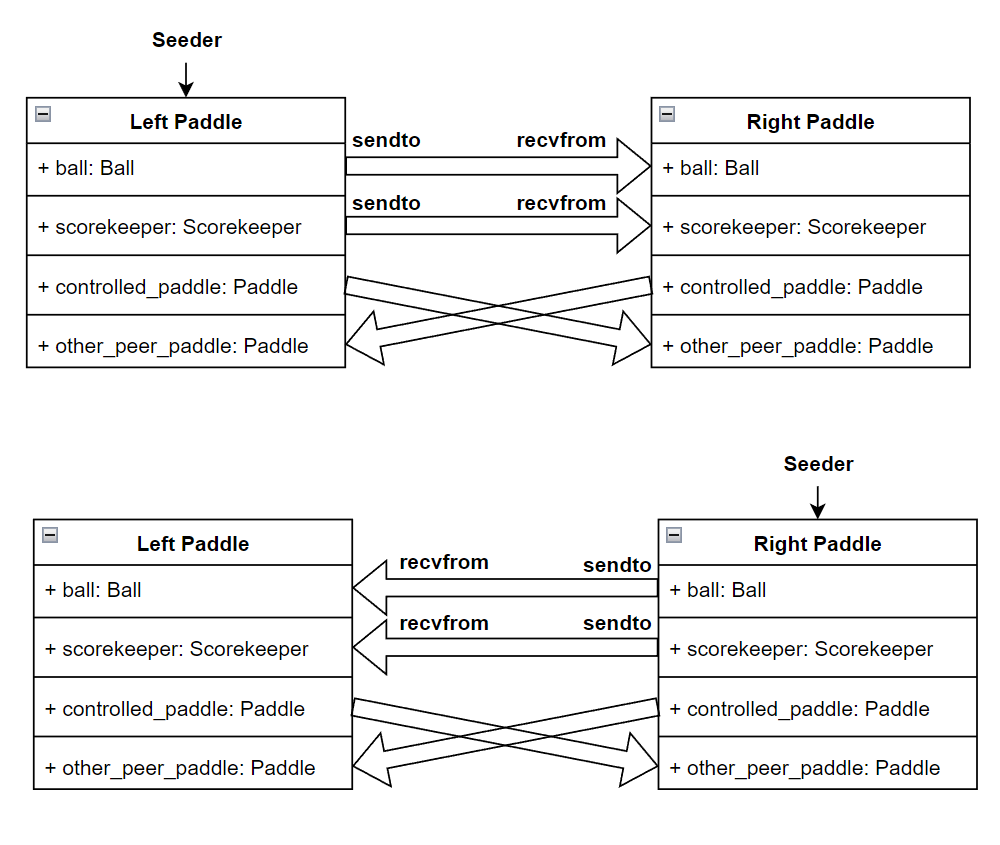
\includegraphics[scale=0.5]{img/schema}
    \caption{Schema dell'architettura}
    \label{fig:schema}
\end{figure}

